% ---
% Arquivo com a revisão bibliográfica do Trabalho de Conclusão de Curso dos alunos
% Gabriel Takaoka Nishimura, Felippe Demarqui Ramos e Vivian Kimie Isuyama 
% da Escola Politécnica da Universidade de São Paulo
% ---
	\chapter{Revisão Bibliográfica}\label{cap-revisao-bibliografica}
	
	Nesse capítulo será feita a verificação do estado atual outros trabalhos.
	
	A única solução comercialmente disponível no mercado é de uma empresa chamada pureLifi, que afirma entregar:

	\begin{itemize}
		\item Estar de acordo com a norma IEEE 802.15.7 - que tem o peso mais alto, já que o escopo principal deste trabalho compreende implementá-la;
		\item Utilização da FPGA para implementar a camada física. As justificativas para o uso desse componente será apresentada nos próximos itens;
		\item Comunicação simplex um a um, que visa garantir a unilateralidade da comunicação entre dois nós, com recepção e transmissão exclusivas a cada uma das partes.
	\end{itemize}

	Antes da publicação da norma 802.15.7 em Setembro de 2011, o Fraunhofer-Gesellschaft conseguiu criar um link de 513 Mbit/s \cite{513mb-fraunhofer} utilizando VLC. A implementação utilizou modulação baseada em DMT (Discrete Multi-Tone) e QAM (Quadrature Amplitude Modulation), assim como técnicas de bit e power loading e clipping simétrico.


	Em 2012, a Scuola Superiore Sant’Anna na Itália provou possível a transmissão de 3.4 Gbit/s com distâncias abaixo de 30cm \cite{3.4g-sant-ana}. O artigo se focou na transmissão de luz com modulação WDM (Wavelength Division Multiplexing) utilizando um LED RGB. Cada comprimento de onda foi então modulado utilizando DMT, que divide o sinal em 512 portadoras, combinadas utilizando QAM.
	
	\begin{figure}[h]
		\caption{\label{figure:bib-rev}Configuração experimental da transmissão WDM. AWG: Gerador de Funções; APD: Fotodiodo de Avalanche}
		\centering
		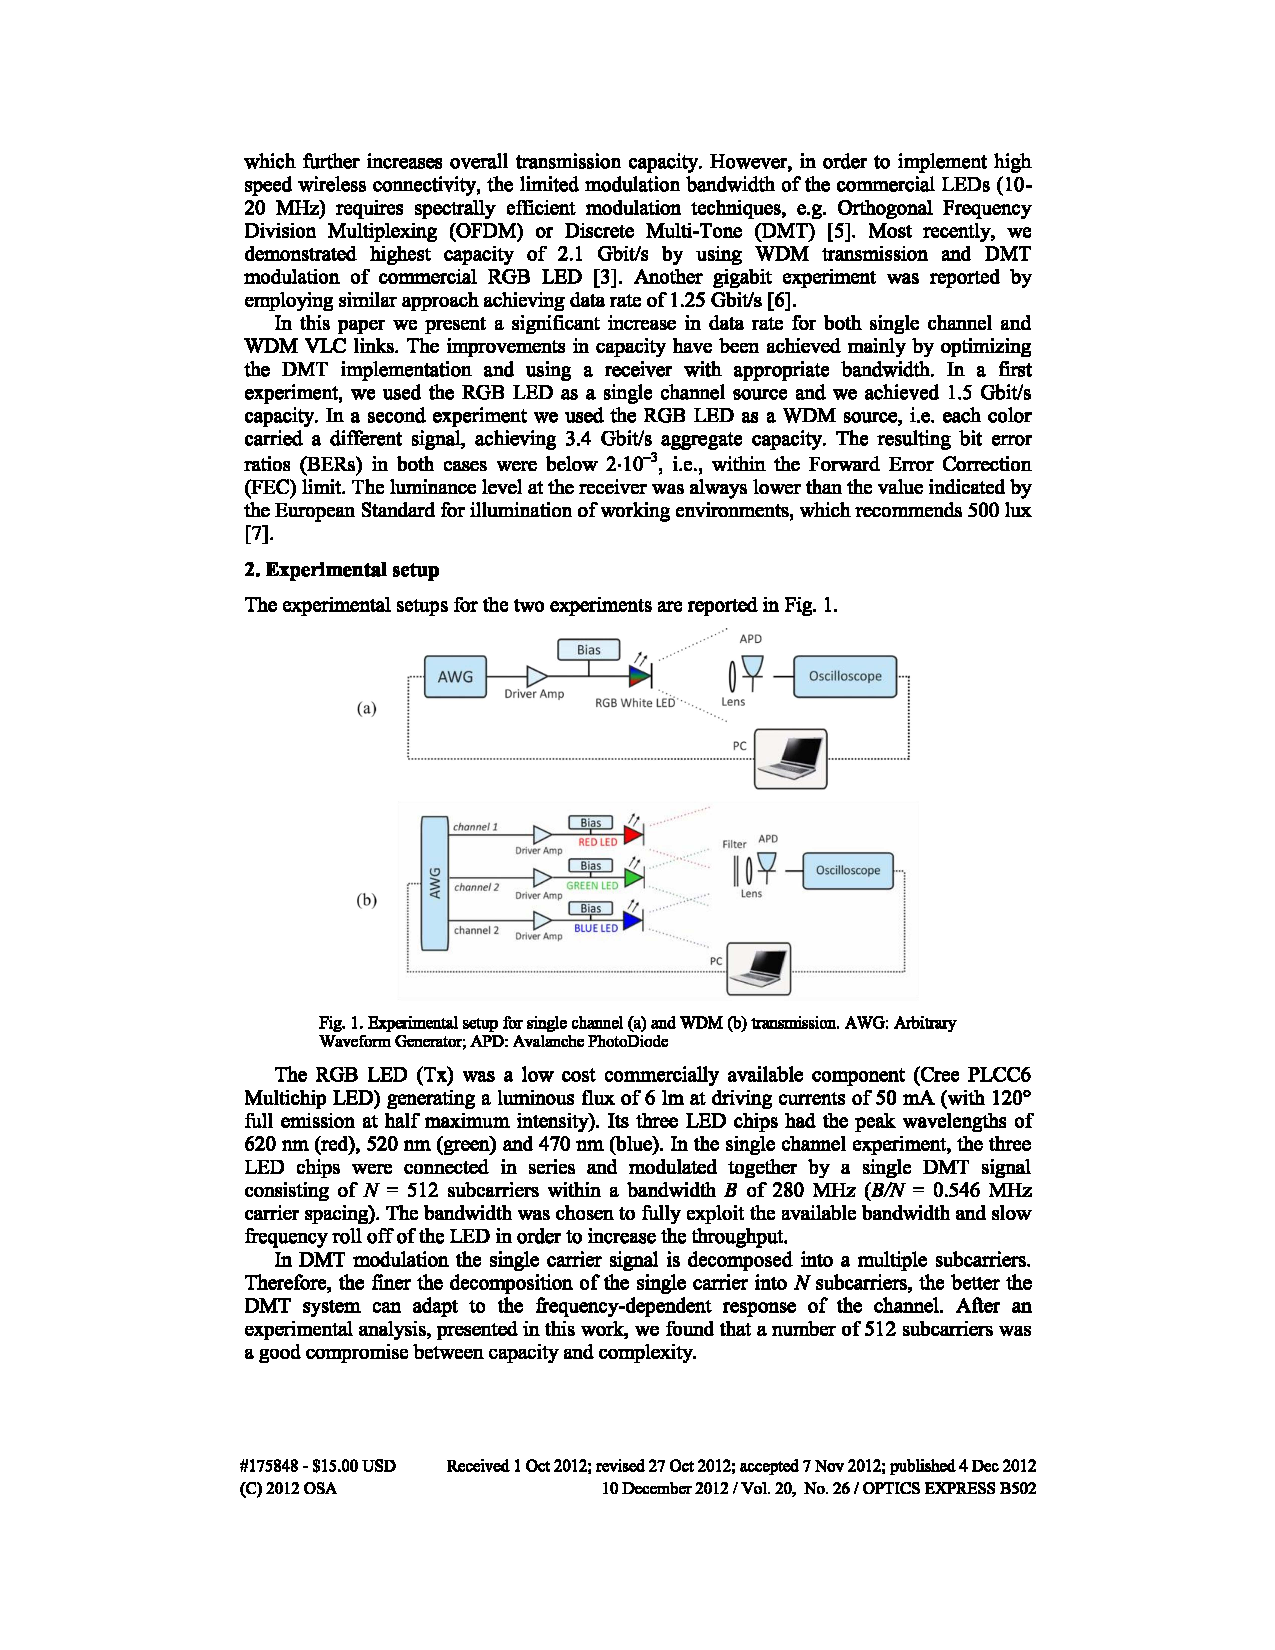
\includegraphics[width=\textwidth, trim={5cm 10cm 7cm 12cm},clip]{sant-ana.pdf}
		\legend{\cite{3.4g-sant-ana}}
	\end{figure}
	
	
	
	
	Abstract: In this paper, we experimentally realized a gigabit-class indoor
	visible light communication system using commercially available RGB
	White LED and exploiting an optimized DMT modulation. We achieved
	data rate of 1.5 Gbit/s with single channel and 3.4 Gbit/s by implementing
	WDM transmission at standard illumination levels. In both experiments, the
	resulting bit error ratios were below the FEC limit. To the best of our
	knowledge, these values are the highest ever achieved in VLC systems. 
	 No artigo de 
	
	\cite{4.5g-fudan}
	Abstract: Inter-symbol interference (ISI) is one of the key problems that
	seriously limit transmission data rate in high-speed VLC systems. To
	eliminate ISI and further improve the system performance, series of
	equalization schemes have been widely investigated. As an adaptive
	algorithm commonly used in wireless communication, RLS is also suitable
	for visible light communication due to its quick convergence and better
	performance. In this paper, for the first time we experimentally demonstrate
	a high-speed RGB-LED based WDM VLC system employing carrier-less
	amplitude and phase (CAP) modulation and recursive least square (RLS)
	based adaptive equalization. An aggregate data rate of 4.5Gb/s is
	successfully achieved over 1.5-m indoor free space transmission with the bit error rate (BER) below the 7percent forward error correction (FEC) limit of 3.8x10−3. To the best of our knowledge, this is the highest data rate ever
	achieved in RGB-LED based VLC systems